\chapter{Methodology}\label{ch:methodology}

\section{Introduction}\label{sec:intro}

In this chapter, the development process for \textbf{Collective} mobile journaling application is explained using the Rapid Application Development (RAD) methodology. Each stage of the developemnt is explained in detail, covering the phases of requirements planning, user design, construction and cutover.

\section{Rapid Application Development (RAD) Methodology}\label{sec:rad}

\begin{figure}[H]
\centering
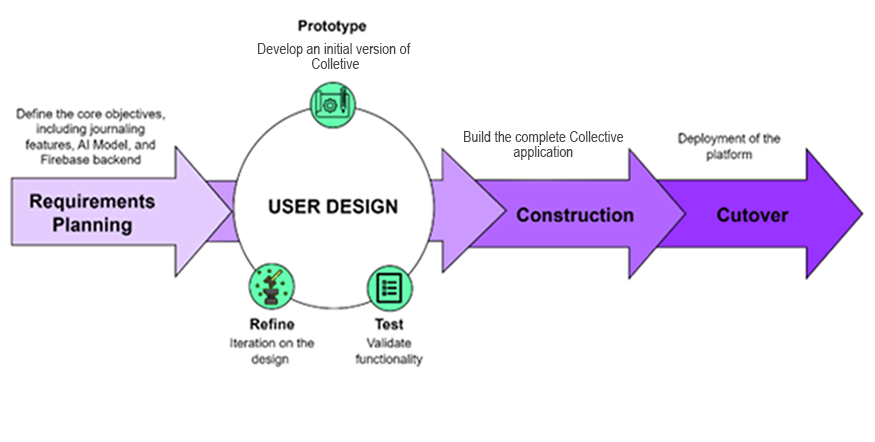
\includegraphics[width=0.8\textwidth]{files/imgs/RAD.png}
\caption{Rapid Application Development (RAD) Methodology Phases}
\label{fig:rad-methodology}
\end{figure}

Rapid Application Development (RAD) is a software development methodology that emphasizes quick development and iteration of prototypes over rigorous planning and testing. It is particularly useful for projects where requirements are expected to evolve or are not fully understood at the outset. The RAD methodology consists of four main phases: requirement planning, user design, construction, and cutover. This model was chosen for the development of the \textbf{Collective} mobile journaling application due to its flexibility and focus on user feedback, which is crucial for creating a user-friendly and effective application. The detais of the project is discussed below:

\section{Requirement planning}\label{sec:requirementPlanning}   

The requirement planning phase is the first step in the RAD methodology, where the project team identifies and defines the requirements of the application. This phase involves gathering information from stakeholders, including potential users, to understand their needs and expectations. The goal is to create a clear and concise set of requirements that will guide the development process.

\subsection{Software Requirements}\label{subsec:softwareRequirements}

The following tables list the software and tools used to develop the \textbf{Collective} mobile journaling application:

\begin{table}[H]
\centering
\caption{Visual Studio Code}
\label{tab:vscode-metadata}
\begin{tabular}{|p{4cm}|p{10cm}|}
\hline
\textbf{Attribute} & \textbf{Details} \\
\hline
Name & Visual Studio Code \\
\hline
Mnemonic & VS Code \\
\hline
Specification Number & N/A \\
\hline
Version Number & 1.101.1 \\
\hline
Source & \url{https://code.visualstudio.com/} \\
\hline
\end{tabular}
\end{table}

\begin{table}[H]
\centering
\caption{Flutter}
\label{tab:flutter-metadata}
\begin{tabular}{|p{4cm}|p{10cm}|}
\hline
\textbf{Attribute} & \textbf{Details} \\
\hline
Name & Flutter \\
\hline
Mnemonic & Flutter SDK \\
\hline
Specification Number & N/A \\
\hline
Version Number & 3.10.0 \\
\hline
Source & \url{https://flutter.dev/} \\
\hline
\end{tabular}
\end{table}

\begin{table}[H]
\centering
\caption{Dart}
\label{tab:dart-metadata}
\begin{tabular}{|p{4cm}|p{10cm}|}
\hline
\textbf{Attribute} & \textbf{Details} \\
\hline
Name & Dart \\
\hline
Mnemonic & Dart SDK \\
\hline
Specification Number & N/A \\
\hline
Version Number & 3.0.0 \\
\hline
Source & \url{https://dart.dev/} \\
\hline
\end{tabular}
\end{table}

\begin{table}[H]
\centering
\caption{Google Chrome}
\label{tab:chrome-metadata}
\begin{tabular}{|p{4cm}|p{10cm}|}
\hline
\textbf{Attribute} & \textbf{Details} \\
\hline
Name & Google Chrome \\
\hline
Mnemonic & Chrome Browser \\
\hline
Specification Number & N/A \\
\hline
Version Number & 114.0.5735.199 \\
\hline
Source & \url{https://www.google.com/chrome/} \\
\hline
\end{tabular}
\end{table}

\begin{table}[H]
\centering
\caption{Microsoft Word}
\label{tab:msword-metadata}
\begin{tabular}{|p{4cm}|p{10cm}|}
\hline
\textbf{Attribute} & \textbf{Details} \\
\hline
Name & Microsoft Word \\
\hline
Mnemonic & MS Word \\
\hline
Specification Number & N/A \\
\hline
Version Number & Office 365 \\
\hline
Source & \url{https://www.microsoft.com/en-us/microsoft-365/word} \\
\hline
\end{tabular}
\end{table}

\begin{table}[H]
\centering
\caption{Microsoft Excel}
\label{tab:msexcel-metadata}
\begin{tabular}{|p{4cm}|p{10cm}|}
\hline
\textbf{Attribute} & \textbf{Details} \\
\hline
Name & Microsoft Excel \\
\hline
Mnemonic & MS Excel \\
\hline
Specification Number & N/A \\
\hline
Version Number & Office 365 \\
\hline
Source & \url{https://www.microsoft.com/en-us/microsoft-365/excel} \\
\hline
\end{tabular}
\end{table}

\begin{table}[H]
\centering
\caption{Draw.io}
\label{tab:drawio-metadata}
\begin{tabular}{|p{4cm}|p{10cm}|}
\hline
\textbf{Attribute} & \textbf{Details} \\
\hline
Name & Draw.io \\
\hline
Mnemonic & Diagram Tool \\
\hline
Specification Number & N/A \\
\hline
Version Number & 20.8.0 \\
\hline
Source & \url{https://app.diagrams.net/} \\
\hline
\end{tabular}
\end{table}

\begin{table}[H]
\centering
\caption{DeepSeek API}
\label{tab:deepseek-metadata}
\begin{tabular}{|p{4cm}|p{10cm}|}
\hline
\textbf{Attribute} & \textbf{Details} \\
\hline
Name & DeepSeek API \\
\hline
Mnemonic & DeepSeek \\
\hline
Specification Number & N/A \\
\hline
Version Number & DeepSeek-V3-0324 \\
\hline
Source & \url{https://platform.deepseek.com/} \\
\hline
\end{tabular}
\end{table}

\subsection{Hardware Requirements}\label{subsec:hardwareRequirements}

The following table lists the hardware requirements necessary for the development and testing of the \textbf{Collective} mobile journaling application. Note that the development is currently focused exclusively on the Android platform, as iOS development requires a macOS machine, which is planned for future work:

\begin{table}[H]
\centering
\caption{Hardware Requirements}
\label{tab:hardware-requirements}
\begin{tabular}{|p{4cm}|p{10cm}|}
\hline
\textbf{Component} & \textbf{Specification} \\
\hline
Processor & Intel Core i5 or equivalent \\
\hline
RAM & 8 GB or higher \\
\hline
Storage & 256 GB SSD or higher \\
\hline
Operating System & Windows 10 \\
\hline
Additional Devices & Android smartphone for testing \\
\hline
\end{tabular}
\end{table}

\subsection{Use Case Diagram}\label{subsec:usecaseDiagram}

The use case diagram for the \textbf{Collective} mobile journaling application illustrates the interactions between the user (Writer) and the system. It highlights the various functionalities provided by the application and their relationships. The diagram is shown below:

\begin{figure}[H]
\centering
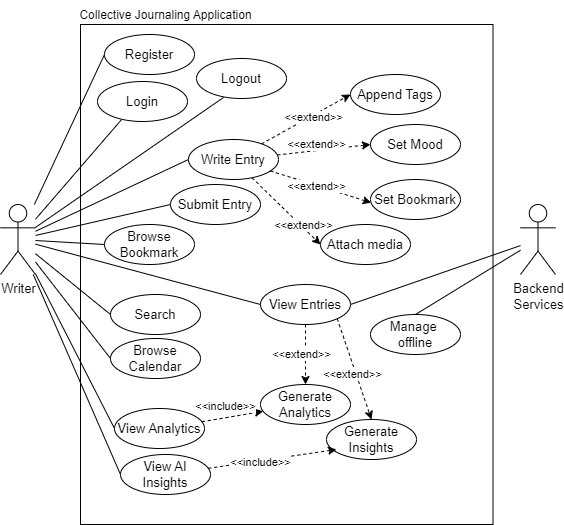
\includegraphics[width=0.8\textwidth]{files/imgs/usecase_diagram.png}
\caption{Use Case Diagram for Collective Mobile Journaling Application}
\label{fig:usecase-diagram}
\end{figure}

\subsection{Use Case Description}\label{subsec:usecaseDescription}

The use case description provides detailed information about the functionalities depicted in the use case diagram. Below is a table summarizing the key use cases:

\begin{table}[H]
\centering
\caption{Use Case Description}
\label{tab:usecase-description}
\begin{tabular}{|p{3cm}|p{5cm}|p{7cm}|}
\hline
\textbf{Actor} & \textbf{Use Case} & \textbf{Use Case Description} \\
\hline
\multirow{15}{*}{Writer} & Register & The writer can register their account by filling in their name, email, and password or use X or Google to register. \\
\cline{2-3}
 & Login & The writer can log in to the application using their registered credentials. \\
\cline{2-3}
 & Logout & The writer can log out of the application when they are done. \\
\cline{2-3}
 & Write Entry & The writer can compose journal entries to record their thoughts and experiences. \\
\cline{2-3}
 & Append Tags & The writer can add tags to their journal entries for better organization. \\
\cline{2-3}
 & Set Mood & The writer can set their mood for each journal entry to reflect their feelings. \\
\cline{2-3}
 & Set Bookmark & The writer can bookmark specific entries for quick access later. \\
\cline{2-3}
 & Attach Media & The writer can attach images or other media to their journal entries. \\
\cline{2-3}
 & Submit Entry & The writer can submit their journal entries to save them in the application. \\
\cline{2-3}
 & Browse Bookmark & The writer can browse through their bookmarked entries. \\
\cline{2-3}
 & View Entries & The writer can view all their saved journal entries. \\
\cline{2-3}
 & Search & The writer can search for specific entries using keywords. \\
\cline{2-3}
 & Browse Calendar & The writer can view their journal entries organized by calendar dates. \\
\cline{2-3}
 & View Analytics & The writer can analyze their journal entries to gain insights into their habits and patterns. \\
\cline{2-3}
 & View AI Insights & The writer can access AI-generated insights based on their journal entries. \\
\hline
\multirow{4}{*}{Backend Services} & View Entries & The system to store and retrieve the writer's journal entries securely. \\
\cline{2-3}
 & Manage Offline & The system to allow the writer to access their entries even when offline. \\
\cline{2-3}
 & Generate Analytics & The system to analyze the writer's journal entries to provide useful statistics. \\
\cline{2-3}
 & Generate Insights & The system to generate insights based on the writer's journal entries to help them understand their patterns. \\
\hline
\end{tabular}
\end{table}

\section{User design}\label{sec:userDesign}

The second phase is the user design phase interacts and participates in the non-technical part design of the project. User feedback is collected to determine the system architecture. During this phase, the design such as user interface, database and others are designated based on the user requirement. User design is a continuous interactive process that allows users to approve the design model that meets their needs. The design process flow for the system is shown in Figure.

\begin{enumerate}
	\item \textbf{Writer}
	%how do i create subitem (roman numeral) below this admin
    \begin{itemize}
        \item[i] \textbf{Register}
    \end{itemize}
\end{enumerate}